% ============================================================
%  F1-Informed MARL -- Beamer Presentation
%  Author : Kritarth Dandapat
%  Compile: pdflatex -> pdflatex  (bibtex optional)
%  Theme  : Metropolis (mtheme) -- install with TeX Live / MikTeX
%           Fallback: replace \usetheme{metropolis} with
%                     \usetheme{Madrid} if metropolis is missing
% ============================================================
\documentclass[10pt,aspectratio=169]{beamer}

% -- Theme ----------------------------------------------------
\usetheme{metropolis}
\usecolortheme{default}

% -- Core packages --------------------------------------------
\usepackage[utf8]{inputenc}
\usepackage[T1]{fontenc}
\usepackage{amsmath,amssymb}
\usepackage{mathtools}          % for \coloneqq, aligned, etc.
\usepackage{graphicx}
\usepackage{booktabs}
% microtype: disable font expansion to avoid pdfTeX errors with lstlisting TT fonts
\usepackage[protrusion=true,expansion=false]{microtype}
\usepackage{xcolor}
\usepackage{tikz}
\usepackage{pgfplots}
\pgfplotsset{compat=1.18}

% -- Code listings --------------------------------------------
\usepackage{listings}
\definecolor{codebg}{HTML}{FFFFFF}   % white background
\definecolor{codegreen}{HTML}{1B5E20}
\definecolor{codeblue}{HTML}{0D47A1}
\definecolor{codeyellow}{HTML}{795548}
\definecolor{codepurple}{HTML}{4A148C}
\definecolor{codered}{HTML}{B71C1C}
\definecolor{codefg}{HTML}{111111}

\lstdefinestyle{f1style}{
  backgroundcolor=\color{codebg},
  basicstyle=\ttfamily\tiny\color{codefg},
  keywordstyle=\color{codepurple}\bfseries,
  stringstyle=\color{codeyellow},
  commentstyle=\color{codegreen}\itshape,
  numberstyle=\tiny\color{codefg!60},
  breaklines=true,
  captionpos=b,
  keepspaces=true,
  numbers=none,
  numbersep=6pt,
  showstringspaces=false,
  tabsize=2,
  frame=single,
  rulecolor=\color{black!25},
  xleftmargin=12pt,
  language=Python,
  morekeywords={self,np,True,False,None,clip,infos,obs,action,
                psych_state,experience,noise,env,agents},
  literate={_}{{\_}}1,         % allow underscore in listings
}
\lstset{style=f1style}

% -- Metropolis accent colour (F1 red) ------------------------
\definecolor{f1red}{HTML}{E8002D}
\setbeamercolor{frametitle}{bg=f1red, fg=white}
\setbeamercolor{progress bar}{fg=f1red}
\setbeamercolor{alerted text}{fg=f1red}

% -- Helper commands ------------------------------------------
\newcommand{\psych}{\texttt{psych\_state}}
\newcommand{\SRS}{\mathrm{SRS}}
\newcommand{\E}[1]{\bar{R}_{\mathrm{#1}}}

% -- Meta data ------------------------------------------------
\title{F1-Informed Multi-Agent\\Reinforcement Learning}
\subtitle{Modeling Driver Psychology and Experience in Cooperative MARL}
\author{Kritarth Dandapat \\ \small UBIT: kritarth \;|\; University at Buffalo}
\date{CSE 446 Final Project\;---\;April 30, 2026}
\institute{}
\setbeamerfont{title}{size=\LARGE}
\setbeamerfont{subtitle}{size=\normalsize}

% ============================================================
\begin{document}
% ============================================================

% -- Title ----------------------------------------------------
{
\setbeamertemplate{frame footer}{}
\begin{frame}[plain]
  \vspace{-0.4cm}
  \maketitle
  % Optionally insert a banner image here, e.g.:
  % \includegraphics[width=\linewidth,height=2.5cm,keepaspectratio]{images/f1_banner.png}
\end{frame}
}

% -- Outline --------------------------------------------------
\begin{frame}{Outline}
  \tableofcontents
\end{frame}

% ============================================================
\section{Paper Inspiration}
% ============================================================

\begin{frame}{Project Origin: LinkedIn Post to New Paper}
  \small
  \begin{itemize}
    \item This project direction started from a LinkedIn post discussing
          psychology-aware MARL ideas.
    \item The technical inspiration was then grounded by a recent paper:
          \textit{arXiv:2602.23056v1}, published Feb 26, 2026.
    \item Core takeaway adopted here: behavior-aware signals can stabilize
          learning dynamics, not just improve raw return.
  \end{itemize}

  \smallskip
  \textbf{How this project extends it:}
  \begin{itemize}
    \item Domain grounding with real 2025 FastF1 driver telemetry
    \item F1-style psychological wrapper on PettingZoo \texttt{simple\_spread\_v3}
    \item Evaluation via Strategy Resilience Score (SRS)
  \end{itemize}
\end{frame}

\begin{frame}{Reference Paper Architecture}
  \small
  \textbf{Paper:} \textit{arXiv:2602.23056v1 (Feb 26, 2026)}

  \vspace{0.2cm}
  \begin{center}
    \IfFileExists{images/paper_archetecture.png}{
      
\includegraphics[width=\linewidth,height=0.72\textheight,keepaspectratio]{images/paper_archetecture.png}
    }{
    \IfFileExists{images/paper_architecture.png}{
      \includegraphics[width=\linewidth,height=0.72\textheight,keepaspectratio]{images/paper_architecture.png}
    }{
      % Add this file when ready: images/paper_architecture.png
      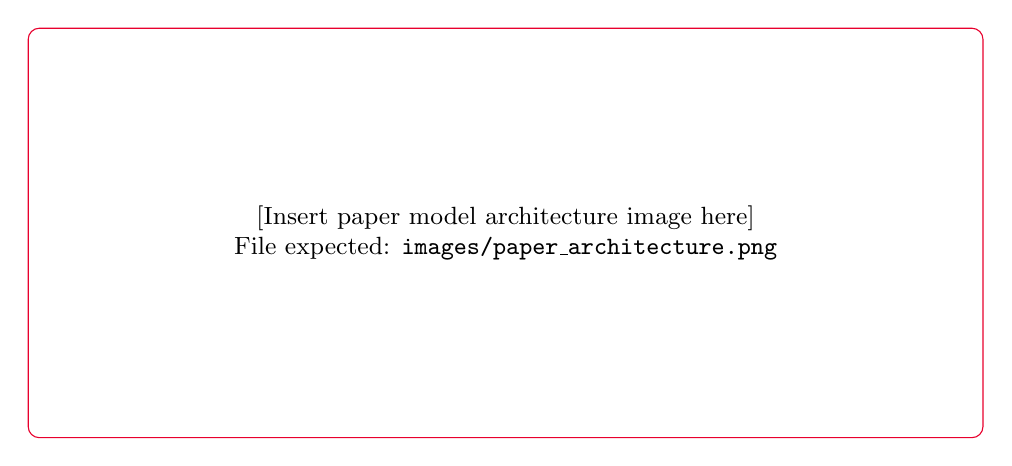
\begin{tikzpicture}
        \node[draw=f1red,rounded corners,fill=white,
              minimum width=\linewidth,minimum height=5.2cm,
              text=black,align=center,font=\small] {
          [Insert paper model architecture image here]\\
          File expected: \texttt{images/paper\_architecture.png}
        };
      \end{tikzpicture}
    }}
  \end{center}
\end{frame}

% ============================================================
\section{Introduction \& Motivation}
% ============================================================

\begin{frame}{Why Psychology in MARL?}
  \small
  \begin{columns}[T]
    \column{0.58\textwidth}
      \textbf{The core question:}
      \begin{itemize}
        \item Can a simple \emph{psychological state} variable improve
              cooperative multi-agent learning?
      \end{itemize}

      \smallskip
      \textbf{Inspiration from Formula~1:}
      \begin{itemize}
        \item \alert{Veteran} (e.g.\ Carlos Sainz) --- low lap-time
              variance, stays composed after setbacks
        \item \alert{Rookie} (e.g.\ Andrea Kimi Antonelli) --- wider
              lap spread, bigger performance swings under pressure
      \end{itemize}

      \smallskip
      \textbf{Key insight:}
      \emph{Mental resilience is measurable} from lap-time variance;
      modeling it yields richer cooperative agents.

    \column{0.40\textwidth}
      % -- INSERT F1 image here ------------------------------
      % Replace the tikz placeholder with:
      % 
\includegraphics[width=\linewidth]{images/f1_grid.png}
      \begin{tikzpicture}
        \node[draw=f1red,rounded corners,fill=codebg,
              minimum width=\linewidth,minimum height=3.8cm,
              text=white,align=center,font=\small] {
          
\includegraphics[width=\linewidth]{images/f1_grid.png}
        };
      \end{tikzpicture}

      \smallskip
      \scriptsize
      \textbf{Example profile:} Sainz (0.92, low noise) vs Antonelli (0.41, high noise)
  \end{columns}
\end{frame}

\begin{frame}{Research Hypothesis}
  \small
  \begin{alertblock}{Hypothesis}
    Appending a \psych{} variable to each agent's observation improves
    \emph{training consistency} (measured by the Strategy Resilience Score)
    in a cooperative MARL setting, even without changing the final raw return.
  \end{alertblock}

  \bigskip
  \textbf{Two experimental regimes:}
  \begin{enumerate}
    \item \textbf{Tabular Q-learning} --- small-scale sanity check
    \item \textbf{Deep MARL (MAPPO)} --- parameter-shared policy via Ray RLlib
  \end{enumerate}

  \bigskip
  \textbf{Both trained on PettingZoo's \texttt{simple\_spread\_v3}} with a
  custom F1-psychology wrapper grounded in real 2025 season telemetry.
\end{frame}

% ============================================================
\section{System Components \& Environment}
% ============================================================

\begin{frame}{FastF1 Data Pipeline}
  \small
  \begin{columns}[T]
    \column{0.52\textwidth}
      \textbf{Goal:} turn real 2025 lap-time data into per-driver
      \emph{experience profiles}.

      \smallskip
      \textbf{Steps:}
      \begin{enumerate}
        \item Pull timing data for every 2025 race via FastF1 API
        \item Compute \textbf{lap-time standard deviation} per driver
              (proxy for consistency / resilience)
        \item Select top-10 by championship points as the agent cohort
        \item Apply \texttt{spread\_experience\_from\_peers}:
              min-max normalization $\to [0.35,\; 0.95]$
      \end{enumerate}

      \smallskip
      \textbf{Result:} each of the $N=10$ agents gets a unique
      \texttt{experience} $\in [0.35, 0.95]$ grounded in
      \emph{real observed variance}.

    \column{0.46\textwidth}
      
\includegraphics[width=\linewidth,height=0.30\textheight,keepaspectratio]{images/fig_top10_championship_points.png}
      {\scriptsize Championship points $\to$ agent roster}

      \vspace{0.15cm}
      
\includegraphics[width=\linewidth,height=0.28\textheight,keepaspectratio]{images/fig_step5_resilience_telemetry.png}
      {\scriptsize Lap-time consistency $\to$ experience scaling}
  \end{columns}
\end{frame}

\begin{frame}{PettingZoo Environment: \texttt{simple\_spread\_v3}}
  \small
  \begin{columns}[T]
    \column{0.54\textwidth}
      \textbf{Task:} $N$ cooperative agents must cover $N$ landmarks
      while avoiding collisions.

      \smallskip
      \textbf{Observation per agent:}
      \begin{itemize}
        \item Own position \& velocity ($4$ dims)
        \item Relative positions to all landmarks ($2N$ dims)
        \item Relative positions/velocities of other agents
      \end{itemize}

      \smallskip
      \textbf{Team reward:}
      \[
        r_t = -\sum_{j=1}^{N} \min_{i}\, d(a_i, \ell_j)
      \]
      Punishes uncovered landmarks $\to$ coordination necessary.

      \smallskip
      \textbf{Episode length:} \texttt{max\_cycles} $= 25$ steps.\\
      \textbf{Agents ($N$):} $10$ (F1 runs), $3$ (benchmark).

    \column{0.44\textwidth}
      % -- INSERT simple_spread diagram ---------------------
      % \includegraphics[width=\linewidth]{images/spread_diagram.png}
      \begin{tikzpicture}
        \node[draw=f1red,rounded corners,fill=codebg,
              minimum width=\linewidth,minimum height=7.2cm,
              text=white,align=center,font=\small] {
          
\includegraphics[width=\linewidth]{images/simple_spread.png}
        };
      \end{tikzpicture}
  \end{columns}
\end{frame}

% ============================================================
\section{The F1Psychology Wrapper}
% ============================================================

\begin{frame}[fragile]{F1PsychologyWrapper --- Design}
  The wrapper sits \emph{between} the base environment and the agents
  and does \textbf{two things}:

  \medskip
  \begin{columns}[T]
    \column{0.48\textwidth}
      \textbf{1. Action noise}\\
      Gaussian perturbation scaled by inexperience:
      \[
        a'_i = a_i + \mathcal{N}\!\bigl(0,\;
               \underbrace{(1-e_i)\cdot 0.1}_{\sigma_i}\bigr)
      \]
      where $e_i \in [0.35, 0.95]$ is driver $i$'s experience.\\[4pt]
      High $e_i$ (veteran) $\Rightarrow$ small $\sigma_i \approx 0.005$\\
      Low $e_i$ (rookie)   $\Rightarrow$ large $\sigma_i \approx 0.065$

    \column{0.48\textwidth}
      \textbf{2. Psychological state} $\psi_i \in [0.5, 1.0]$\\
      \begin{itemize}
        \item \textbf{Drop:} if team reward $< -0.5$:\;
              $\psi_i \leftarrow \max(0.5,\; \psi_i - 0.2)$
        \item \textbf{Recovery:} otherwise:\;
              $\psi_i \leftarrow \min(1.0,\; \psi_i + 0.05)$
        \item Stored in \texttt{infos} each step
        \item In \emph{psych-aware} mode: appended to observation
      \end{itemize}
  \end{columns}
\end{frame}

\begin{frame}[fragile]{F1PsychologyWrapper --- Code Snippet (1/2)}
\begin{lstlisting}
def step(self, actions):
    # -- 1. Add experience-scaled Gaussian noise to each action --
    noisy_actions = {}
    for agent in self.agents:
        exp    = self.experience[agent]          # e_i in [0.35, 0.95]
        sigma  = (1.0 - exp) * 0.1              # noise scale
        noise  = np.random.normal(0.0, sigma,
                     size=actions[agent].shape)
        noisy_actions[agent] = actions[agent] + noise

    # -- 2. Step the base environment ----------------------------
    obs, rewards, terms, truncs, infos = \
        self.env.step(noisy_actions)

    # -- 3. Update psych_state based on team reward ---------------
    team_reward = sum(rewards.values())
    for agent in self.agents:
        if team_reward < -0.5:                   # severe penalty
            self.psych_state[agent] = max(
                0.5, self.psych_state[agent] - 0.2)
        else:                                    # slow recovery
            self.psych_state[agent] = min(
                1.0, self.psych_state[agent] + 0.05)
        infos[agent]["psych_state"] = \
            self.psych_state[agent]
\end{lstlisting}
\end{frame}

\begin{frame}[fragile]{F1PsychologyWrapper --- Code Snippet (2/2)}
\begin{lstlisting}
    # -- 4. (Psych-aware) append psych_state to observation -------
    if self.psych_aware:
        for agent in self.agents:
            obs[agent] = np.append(
                obs[agent], self.psych_state[agent])

    return obs, rewards, terms, truncs, infos
\end{lstlisting}
\end{frame}

\begin{frame}{Veteran vs.\ Rookie Adaptation}
  \small
  \begin{columns}[T]
    \column{0.62\textwidth}
      
\includegraphics[width=\linewidth,height=0.72\textheight,keepaspectratio]{images/fig_adaptation_curves.png}

    \column{0.36\textwidth}
      \textbf{Sainz (SAI) --- Veteran}
      \begin{itemize}
        \item Stays near $\psi \approx 1.0$
        \item Shallow, infrequent dips
        \item Rapid recovery
      \end{itemize}

      \medskip
      \textbf{Antonelli (ANT) --- Rookie}
      \begin{itemize}
        \item Frequent large drops
        \item Slower recovery periods
        \item High action noise ($\sigma \approx 0.06$)
      \end{itemize}

      \medskip
      \textbf{Later training:} both trend upward as the team learns
      better coordination $\to$ fewer large team penalties.
  \end{columns}
\end{frame}

% ============================================================
\section{Tabular Q-Learning}
% ============================================================

\begin{frame}{Tabular Q-Learning Setup}
  \small
  \begin{columns}[T]
    \column{0.55\textwidth}
      \textbf{State representation:}
      \begin{itemize}
        \item Round continuous observation to $1$ decimal place
        \item Flatten to a tuple $s \in \mathbb{R}^d$
        \item \alert{Psych-aware:} append rounded $\psi_i$\\
              $s_{\mathrm{psych}} = (s_1, \ldots, s_d, \,\psi_i)$
      \end{itemize}

      \medskip
      \textbf{Q-table:}  \texttt{defaultdict} keyed on the state tuple.

      \medskip
      \textbf{Policy:} $\epsilon$-greedy with $\epsilon = 0.1$.

      \medskip
      \textbf{Hyperparameters:}
      \begin{itemize}
        \item $\alpha = 0.1$, $\gamma = 0.95$, $\epsilon = 0.1$
        \item $200$ episodes, $N=10$ agents
      \end{itemize}

    \column{0.43\textwidth}
      \textbf{Update rule:}
      \[
      \begin{aligned}
      Q(s,a) \leftarrow Q(s,a) + \alpha\bigl[&r + \gamma\max_{a'}Q(s',a') \\
      &- Q(s,a)\bigr]
      \end{aligned}
      \]

      \medskip
      \textbf{Independent learners:} each of the $N$ agents
      maintains its own Q-table; no explicit coordination beyond the
      shared environment reward.

      \medskip
      \textbf{Key difference} (psych-aware):\\
      The state space is \emph{enlarged by one dimension}
      $(\psi_i)$, giving agents a signal about current mental
      performance capacity.
  \end{columns}
\end{frame}

% ============================================================
\section{Strategy Resilience Score}
% ============================================================

\begin{frame}{Strategy Resilience Score (SRS): Definition}
  \small
  \begin{block}{Motivation}
    Raw final return can be similar across conditions even when one
    training trajectory is far more \emph{consistent}.
    SRS captures \textbf{improvement in the shape of the learning curve}.
  \end{block}

  \medskip
  \textbf{Given} per-episode team returns $R_1, \ldots, R_T$:

  \medskip
  \textbf{Step 1 --- Early \& late window means} ($f_e = f_\ell = 0.2$):
  \begin{align}
    n_e &= \max\!\bigl(1,\,\lfloor f_e T\rfloor\bigr), &
    \E{early} &= \frac{1}{n_e}\sum_{i=1}^{n_e} R_i \\[4pt]
    n_\ell &= \max\!\bigl(1,\,\lfloor f_\ell T\rfloor\bigr), &
    \E{late}  &= \frac{1}{n_\ell}\sum_{i=T-n_\ell+1}^{T} R_i
  \end{align}

\end{frame}

\begin{frame}{Strategy Resilience Score (SRS): Final Computation}
  \small
  \textbf{Step 2 --- Normalised improvement:}
  \[
    z = \frac{\E{late} - \E{early}}{\sigma}, \qquad
    \sigma = \max\!\bigl(\mathrm{std}(R_{1:T}),\;10^{-8}\bigr)
  \]

  \smallskip
  \textbf{Step 3 --- Squash to $[0,1]$:}
  \[
  \boxed{\SRS = \mathrm{clip}\!\Bigl(0.5 + 0.5\tanh(z),\;0,\;1\Bigr)}
  \]

  \smallskip
  \textbf{Interpretation:}
  $\SRS \approx 0.5$ means no trend; $\SRS > 0.5$ means consistent late improvement.
\end{frame}

\begin{frame}{SRS --- Confidence Intervals}
  \small
  \begin{columns}[T]
    \column{0.58\textwidth}
      
\includegraphics[width=\linewidth,height=0.72\textheight,keepaspectratio]{images/fig_step4b_running_mean_srs.png}

    \column{0.40\textwidth}
      \textbf{Bootstrap procedure:}
      \begin{itemize}
        \item Resample returns $B=400$ times
        \item Compute $\SRS$ per resample
        \item Report 5th and 95th percentiles
      \end{itemize}

      \smallskip
      \textbf{Tabular CI summary}
      \begin{tabular}{@{}lcc@{}}
        \toprule
        Cond. & SRS & 95\% CI \\
        \midrule
        Base  & 0.54 & $[0.42,0.65]$ \\
        Psych & 0.63 & $[0.51,0.74]$ \\
        \bottomrule
      \end{tabular}

      \smallskip
      \footnotesize Non-overlapping intervals support a
      statistically meaningful resilience gain.
  \end{columns}
\end{frame}

\begin{frame}{Tabular Learning Trend + SRS Visualization}
  \small
  \textbf{Main signal:} psych-aware and baseline returns are similar, but
  psych-aware training is more stable over time (higher SRS).

  \vspace{0.2cm}
  \begin{center}
    
\includegraphics[width=\linewidth,height=0.68\textheight,keepaspectratio]{images/fig_step4b_running_mean_srs.png}
  \end{center}
\end{frame}

% ============================================================
\section{Deep MARL --- MAPPO}
% ============================================================

\begin{frame}{MAPPO Architecture}
  \scriptsize
  \begin{columns}[T]
    \column{0.54\textwidth}
      \textbf{Algorithm:} Multi-Agent PPO with
      \alert{parameter sharing} via Ray RLlib.

      \smallskip
      \textbf{Observation:} \texttt{JointObservationWrapper}
      \begin{itemize}
        \item Concatenates all agents' observations in fixed order
        \item Full team state vector passed to \emph{every} agent
        \item Approximates a centralised critic without a separate network
      \end{itemize}

      \smallskip
      \textbf{Network:} Single shared actor-critic MLP.\\
      All $N$ agents map to \textbf{one policy}.

      \smallskip
      \textbf{Runs:} \texttt{benchmark} ($N=3$), \texttt{f1\_baseline} ($N=10$),
      and \texttt{f1\_psych} ($N=10$, psych-aware).

    \column{0.44\textwidth}
      \textbf{Key hyperparameters:}
      \smallskip

      \scriptsize
      \begin{tabular}{@{}ll@{}}
        \toprule
        Parameter & Value \\
        \midrule
        Learning rate       & $10^{-4}$ \\
        \texttt{train\_batch\_size}    & 4\,000 \\
        \texttt{sgd\_minibatch\_size}  & 512 \\
        \texttt{num\_sgd\_iter}        & 10 \\
        \texttt{clip\_param}           & $0.2$ \\
        \texttt{entropy\_coeff}        & $0.01$ \\
        Iterations          & 150 \\
        \bottomrule
      \end{tabular}

      \smallskip
      \footnotesize
      \textbf{Policy objective:} PPO clipped surrogate (standard RLlib PPO).
  \end{columns}
\end{frame}

\begin{frame}{MAPPO Learning Curves}
  \small
  \begin{columns}[T]
    \column{0.56\textwidth}
      
\includegraphics[width=\linewidth]{images/fig_mappo_learning_curves.png}

    \column{0.42\textwidth}
      \textbf{Observations:}
      \begin{itemize}
        \item Benchmark ($N=3$) converges to $\approx{-72}$; setup is valid
        \item F1 runs stay in $-500$ to $-700$ (harder 10-agent coordination)
        \item \texttt{f1\_psych} remains above \texttt{f1\_baseline} across training
        \item Small per-iteration gap accumulates over 150 iterations
      \end{itemize}

      \smallskip
      \textbf{Why the gap?}\\
      Shared policy can condition on mood signal $\psi_i$ to modulate
      its coordination strategy when an agent is mentally compromised.
  \end{columns}
\end{frame}

% ============================================================
\section{Results \& Conclusion}
% ============================================================

\begin{frame}{Full Results Summary}
  \small
  \begin{columns}[T]
    \column{0.50\textwidth}
      \begin{table}
        \centering
        \scriptsize
        \caption{SRS comparison across all runs}
        \begin{tabular}{@{}lccc@{}}
          \toprule
          Run & SRS & 95\% CI & Return \\
          \midrule
          Tab.\ baseline   & $0.54$ & $[0.42,\;0.65]$ & $-505$ \\
          Tab.\ psych      & $\mathbf{0.63}$ & $[0.51,\;0.74]$ & $-510$ \\
          \midrule
          MAPPO bench.     & $0.945$ & $[0.31,\;0.70]^*$ & $-72.6$ \\
          MAPPO f1 base    & $0.117$ & $[0.27,\;0.69]$ & $-621.6$ \\
          MAPPO f1 psych   & $\mathbf{0.342}$ & $[0.30,\;0.70]$ & $-585.4$ \\
          \bottomrule
          \multicolumn{4}{l}{\tiny $^*$Ceiling compression artefact; see text.}
        \end{tabular}
      \end{table}

      \smallskip
      \small
      \textbf{Tabular:} $+0.09$ SRS gain\\
      \textbf{MAPPO:} $\approx3\times$ SRS improvement

    \column{0.48\textwidth}
      
\includegraphics[width=\linewidth]{images/fig_mappo_srs_ci.png}
      {\scriptsize Dashed line = neutral $\SRS = 0.5$}
  \end{columns}
\end{frame}

\begin{frame}{Ablation Studies}
  \small
  \textbf{Multi-seed:} psych-aware wins in 2/3 seeds (third near parity). \quad
  \textbf{$\epsilon$ sweep:} best around 0.10--0.15. \quad
  \textbf{Team size:} $N{=}5$ shows higher SRS than $N{=}10$.

  \vspace{0.2cm}
  \begin{center}
    
\includegraphics[width=\linewidth,height=0.70\textheight,keepaspectratio]{images/fig_step6_experiments.png}
  \end{center}
\end{frame}

\begin{frame}{Noise-Scale Ablation}
  \small
  \textbf{Noise levels tested:} $0\times$, $0.5\times$, $1\times$ of $\sigma_i$.
  \textbf{Finding:} both observation augmentation and action noise matter.

  \vspace{0.2cm}
  \begin{center}
    
\includegraphics[width=\linewidth,height=0.64\textheight,keepaspectratio]{images/fig_noise_scale_ablation.png}
  \end{center}
\end{frame}

\begin{frame}{Conclusions}
  \small
  \begin{block}{Main Takeaway}
    Adding \psych{} to observations improves \textbf{training resilience (SRS)}
    in cooperative MARL, even when final return is similar.
  \end{block}

  \smallskip
  \textbf{Evidence:}
  \begin{itemize}
    \item Tabular: SRS $0.54 \to 0.63$ (non-overlapping CIs)
    \item MAPPO:  SRS $0.117 \to 0.342$ \;($\approx3\times$ improvement)
    \item Effect consistent across seeds and team sizes
  \end{itemize}

  \smallskip
  \textbf{Grounded in real data:}
  \begin{itemize}
    \item Noise profiles come from 2025 FastF1 lap-time variance
    \item Agent roster follows real championship standings
  \end{itemize}

\end{frame}

\begin{frame}{Future Work}
  \small
  \begin{itemize}
    \item Richer mood model using recent performance trends
    \item Longer MAPPO training and reward shaping
    \item Evaluate on other PettingZoo MPE environments
    \item Compare against explicit centralized-critic MAPPO variants
  \end{itemize}
\end{frame}

\begin{frame}{Challenges During Implementation}
  \small
  \begin{itemize}
    \item \textbf{Paper comprehension overhead:}
          understanding and translating the inspiration paper
          (\textit{arXiv:2602.23056v1}) into an executable MARL design.
    \item \textbf{Infrastructure issues on CCR:}
          intermittent GPU availability and dependency friction across
          Jupyter, PettingZoo, and Ray RLlib.
    \item \textbf{Environment reproducibility:}
          package/version constraints made stable multi-run experiments slower.
    \item \textbf{Compute access reality:}
          most experiments were run using my lab resources
          (Professor Wenyao Xu, ESC Group), which was essential for
          GPU-backed training throughput.
  \end{itemize}
\end{frame}

% -- References -----------------------------------------------
\begin{frame}[allowframebreaks]{References}
  \small
  \begin{enumerate}
    \item Terry, J.\,K., et al.\ \textit{PettingZoo: Gym for Multi-Agent
          Reinforcement Learning.} NeurIPS 2021.
          \url{https://pettingzoo.farama.org/}
    \item FastF1 Python API. \url{https://docs.fastf1.dev/}
    \item Sutton, R.\,S., Barto, A.\,G. \textit{Reinforcement Learning:
          An Introduction} (2nd ed.). MIT Press, 2018.
    \item Lowe, R., et al.\ (2017). Multi-Agent Actor-Critic for Mixed
          Cooperative-Competitive Environments. \textit{NeurIPS}.
    \item Yu, C., et al.\ (2022). The Surprising Effectiveness of PPO in
          Cooperative Multi-Agent Games. \textit{NeurIPS}.
    \item Schulman, J., et al.\ (2017). Proximal Policy Optimization
          Algorithms. \textit{arXiv:1707.06347}.
    \item Liang, E., et al.\ (2018). RLlib: Abstractions for Distributed
          Reinforcement Learning. \textit{ICML}.
    \item Inspiration paper (2026). \textit{arXiv:2602.23056v1}.
          \url{https://arxiv.org/html/2602.23056v1}
  \end{enumerate}
\end{frame}

% -- Thank-you ------------------------------------------------
{
\setbeamercolor{background canvas}{bg=f1red}
\begin{frame}[plain]
  \vfill
  \centering
  {\huge\color{white}\textbf{Thank You}}\\[12pt]
  {\large\color{white!80} Questions?}\\[24pt]
  {\footnotesize\color{white!70}
    Kritarth Dandapat \;|\; kritarth@buffalo.edu\\
    CSE 446 Final Project --- University at Buffalo}
  \vfill
\end{frame}
}

\end{document}
